% Chapter Template

\chapter{Resultados} % Main chapter title

\label{Chapter4} % Change X to a consecutive number; for referencing this chapter elsewhere, use \ref{ChapterX}

%----------------------------------------------------------------------------------------
%	SECTION 1
%----------------------------------------------------------------------------------------

\section{Resultados}
\label{sec: Resultados}

\subsection{Resultados del CFAR a ensayos con marcos de prueba}

\subsubsection{CFAR. Ensayo 1}
\label{Subsec:CFAR. Ensayo 1}

Se simuló el \textit{test bench} del CFAR para un intervalo de tiempo comprendido entre $0 us$ y $121 us$. La señal de estímulo del video de entrada se creó con las siguientes características para emular de manera aproximada una señal real:

\begin{itemize}
\item
Valor bajo equivalente al piso de ruido durante todo el periodo, excepto durante un pequeño intervalo de tiempo en la que adquiere un valor mayor. Se eligió como valor bajo \texttt{10000000000000} debido a que el conversor de alta velocidad es de 14-bit signado y el valor mencionado corresponde al cero. Físicamente el piso de ruido era cercano a cero. El valor de amplitud del pulso de video se eligió \texttt{10111011100000} como valor cercano al $50\%$ del rango de operación.


\item
Periódica de periodo suficientemente largo para que exista un solo pulso en el intervalo de tiempo que comprende la totalidad de celdas CFAR. La totalidad de las celdas CFAR generan un retardo indicado en la ecuación \ref{Eq:delay_cfar}, donde $N_{rc}$ es igual al número total de las celdas de referencia (128), $N_{gc}$ es igual al número total de las celdas de guarda (10) y $N_t$ es igual a el número total de las celdas bajo testeo (1).

\end{itemize}

\begin{equation}
T_{clk} *(N_{rc} + N_{gc} + N_t) =  0,8 us * 139 = 111,2 us
\label{Eq:delay_cfar}
\end{equation}



Se introdujo dos señales de reloj de diferentes periodos, de valores similares a los periodos reales. El primero para comandar la transferencia de datos entre las celdas CFAR y el segundo para realizar la comparación entre el umbral generado por el CFAR y el valor de video de la celda bajo testeo.

Se adoptó como valor inicial de multiplicador el valor $15784$ debido a que en ensayos preliminares con señal de radar real se observó que el mismo era un valor apropiado para determinar un rango útil de multiplicador.

En resumen, se introdujo los siguientes estímulos:
\begin{itemize}
\item Señal de reloj 1 de 800 ns de periodo.
\item Señal de reloj 2 de 20 ns de periodo.
\item Señal de algoritmo en "00". Correspondiente al algoritmo CA-CFAR.
\item Señal de video de entrada \texttt{video\_cf\_tb} de \texttt{14\-bit} tipo unsigned, periódica de periodo igual a 61 us, con valor \texttt{10000000000000} (8192 en sistema decimal) durante 60 us y \texttt{10111011100000} (12000 en sistema decimal) durante 1 us.
\item Señal de habilitación con valor permante en '1' lógico (siempre habilitado).
\item Señal de reset con valor permanente en '0' lógico (nunca resetea).
\item Señal de multiplicador inicializado en 15784 con incremento de una unidad en cada flanco ascendente del reloj 1.
\end{itemize}

El resultado de este ensayo se ilustra en la figura \ref{fig:cfar_ensayo_1}. Un acercamiento de la señal de multiplicador se ilustra en la figura \ref{fig:cfar_ensayo_1_zoom_multiplicador}.

\begin{figure}
\centering
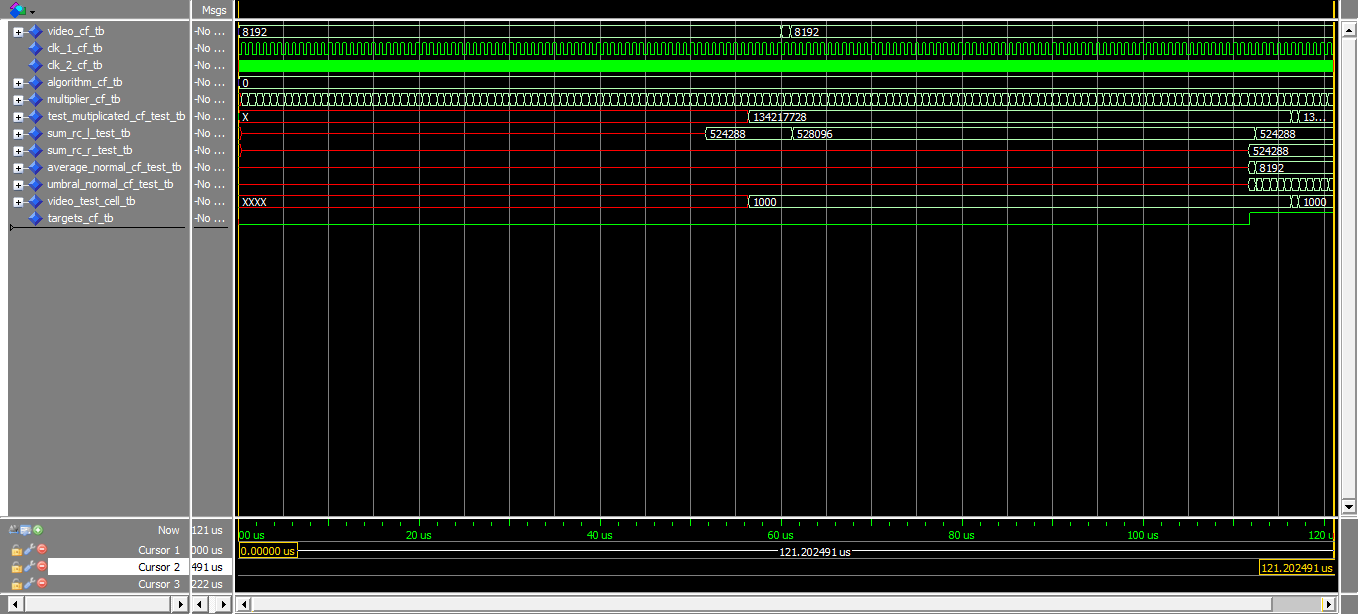
\includegraphics[scale=0.52, angle=270]{./Figures/cfar_ensayo_1.png}
\caption{CFAR. Ensayo 1 con \textit{testbench}}
\label{fig:cfar_ensayo_1}
\end{figure}

\begin{figure}
\centering
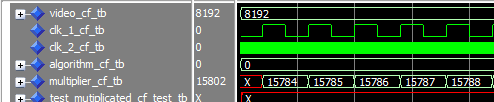
\includegraphics[scale=1]{./Figures/cfar_ensayo_1_zoom_multiplicador.png}
\caption{Acercamiento del ensayo 1. Variación del multiplicador}
\label{fig:cfar_ensayo_1_zoom_multiplicador}
\end{figure}



Se observó lo siguiente:

\begin{itemize}
\item
Las señales de estímulos se generaron adecuadamente.

\item
% (0.8*N)-0.4 = delay. N es el número de flanco.
Desde $0$ a $56,42 us$ la salida de la celda test estuvo indefinida. Esto se debe a la cantidad de flancos de reloj necesarios del reloj 1 para que el dato llegue a la celda  test, debiendo pasar antes por 64 celdas de referencia, 5 celdas de guarda y la propia celda test. Una vez que se actualizó la salida del la celda test se añade otro retraso interno al cfar, de un periodo del reloj 2, dado por el componente comparador, como se ilustra en la figura \ref{fig:cfar_ensayo_1_zoom_test_cell}. Este retraso debido al comparador se debe al tiempo que invierte el componente en realizar los cálculos de promediación y comparación para determinar si el video almacenado en la celda bajo testeo supera o no el umbral, la actualización de los datos de entrada y salida de este componente son dados en los flancos descendentes del reloj 2 para crear un desfase de $180º$ respecto del reloj 1 y asegurar la estabilidad del dato. Por último, se suma un retardo adicional de un periodo del reloj 1, correspondiente al registro de salida del cfar.

\begin{figure}
\centering
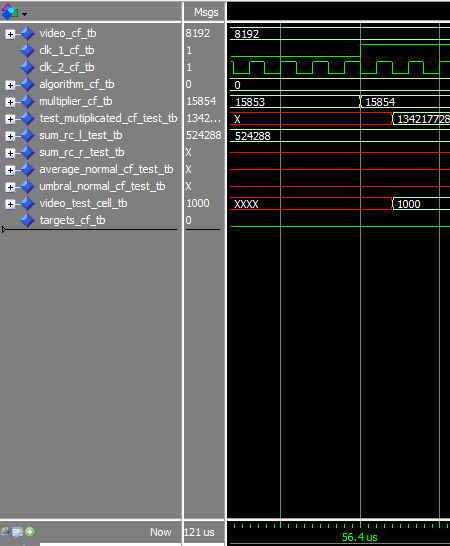
\includegraphics[scale=1]{./Figures/cfar_ensayo_1_zoom_test_cell.png}
\caption{CFAR.Ensayo 1. Acercamiento al tiempo $t=56.4 us$}
\label{fig:cfar_ensayo_1_zoom_test_cell}
\end{figure}


\item
Las señales de salida \textit{test\_mutiplicated\_cf\_test\_tb} y \textit{o\_test\_mutiplicated\_cfar}, actualizaron sus valores simultáneamente. El primero corresponde a la salida de la celda test; se actualizó al valor \texttt{134217728}, correspondiente a una corrección dada por la ecuación \ref{Eq:corrección_test_cell}, donde: $V_{tc corregido}$ es la corrección sobre el valor de video almacenado en la celda test, $V_{tc}$ es el valor de video almacenado en la celda test y $2^{14}$ es la resolución del ADC de alta velocidad. La segunda señal corresponde al puerto de salida del cfar de la celda test; se actualizó al valor \texttt{1000} (en sistema binario) debido a que representa en el sistema binario a una porción del valor de la celda test. Ocurre algo similar luego de $60 us$ cuando llega el pulso de video a la celda test.

\begin{equation}
V_{tc   corregido} = V_{tc} * 2^{14} = 8192 * 16384 = 134217728
\label{Eq:corrección_test_cell}
\end{equation}

\item
Desde 0 a 51,61 us la salida de la suma de todas las celdas de referencias ubicadas a la izquierda de la celda test, \texttt{sum\_rc\_l\_test\_tb}, se encuentra indefinida. Este retraso se ilustra en la figura \ref{fig:cfar_ensayo_1_zoom_sum_rc} y, como se indica en la ecuación \ref{Eq:delay_suma_rc_l}, se debe a la cantidad de flancos de reloj 1 necesarios para que el dato pase por todas las celdas y sea posible realizar la suma de sus valores almacenados, más un retraso adicional de 1 periodo del reloj 2, debido al registro de salida incorporado dentro del cfar. Luego de ese intervalo de tiempo la suma se actualizó al valor $8192 * 64 = 524288$, debido a que todas las celdas de referencia ubicadas a la izquierda de la celda test almacenaron el valor constante de $8192$. Se puede realizar un análisis similar para la celda de referencia ubicada a la derecha de la celda test, que dejó de estar indefinida a los $111,6 us$ debido al tiempo necesario para superar el retardo generado por sus celdas de referencia y las celdas anteriores, como se indica en la ecuación \ref{Eq:delay_suma_rc_r}.

\begin{figure}
\centering
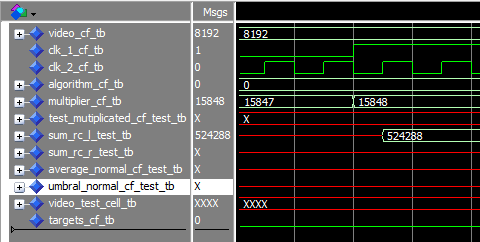
\includegraphics[scale=1]{./Figures/cfar_ensayo_1_zoom_sum_rc.png}
\caption{Acercamiento del ensayo 1. Detalle de la suma de salida de la celda de referencia izquierda}
\label{fig:cfar_ensayo_1_zoom_sum_rc}
\end{figure}

\begin{equation}
T_{clk 1} * N_{rc} - \dfrac{T_clk_1}{2} + \dfrac{T_clk_2}{2} = 0,8 us * 64 - 0,4 us + 0,02 us= 56,4 us
\label{Eq:delay_suma_rc_l}
\end{equation}


\begin{equation}
0,8 us *(64 + 64 + 5 + 5 + 1) + 0,4 us = 111,6 us
\label{Eq:delay_suma_rc_r}
\end{equation}

\item
A los 111,62 us, medio periodo del reloj 2 luego de haber quedado definido la sumas de la celda de referencia izquierda y, por tanto, teniendo disponible la suma de ambas celdas de referencia, se crea el promedio normal, como se ilustra en la figura \ref{fig:cfar_ensayo_1_zoom_umbral}. El promedio normal está compuesto por la suma de ambas celdas de referencia dividido 128, valor correspondiente a la cantidad total de celdas de ambas celdas de referencia. También en la figura\ref{fig:cfar_ensayo_1_zoom_umbral} se observó que $60 ns$ después de que el promedio normal (retraso necesario para efectuar el cálculo), la señal de salida del umbral normal adquirió un valor definido. El mismo adquierió el último valor de la multiplicación del promedio por el multiplicador, como se indica en la ecuación \ref{Eq:Ecuación del umbral normal}. A partir de ese momento, su valor creció en cada flanco ascendente del reloj 1 debido a que se encuentra afectado por el multiplicador.

\begin{figure}
\centering
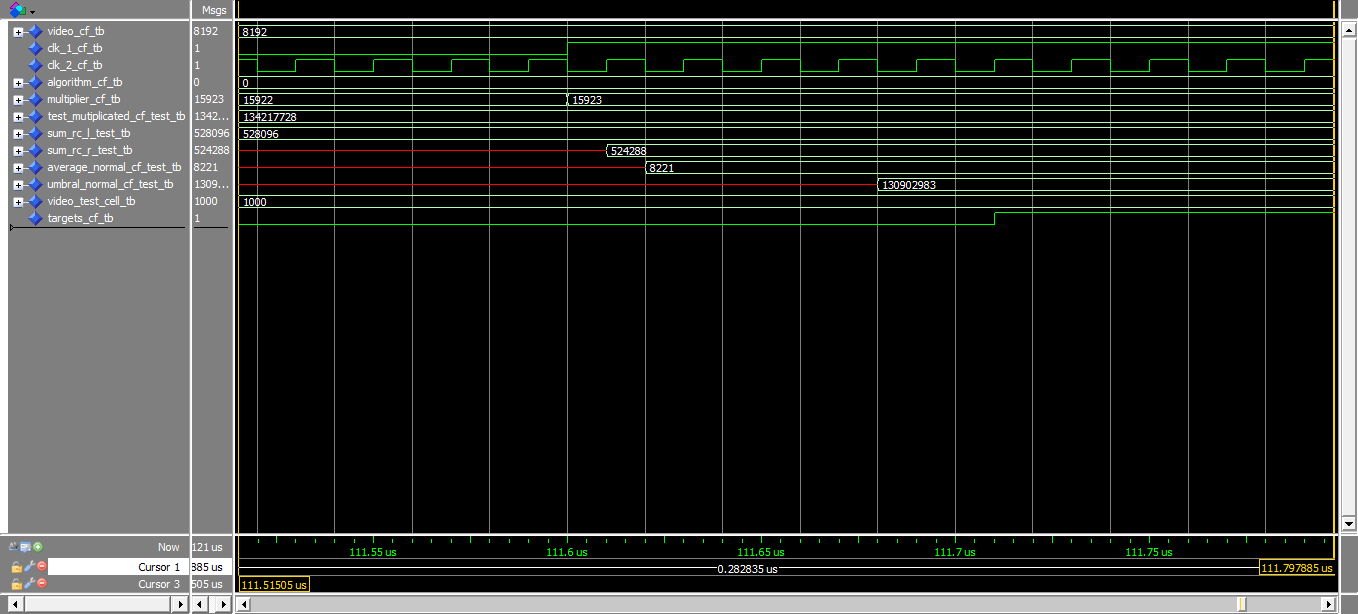
\includegraphics[scale=0.52, angle=270]{./Figures/cfar_ensayo_1_zoom_umbral.png}
\caption{CFAR. Ensayo 1 con \textit{testbench}, zoom alrededor de los 111,65 us}
\label{fig:cfar_ensayo_1_zoom_umbral}
\end{figure}

\begin{equation}
umbral_{normal} = promedio_{normal} * multiplicador = 8221 * 15923 = 130902983
\label{Eq:Ecuación del umbral normal}
\end{equation}

\item
Se observó a partir de los $111,68 us$ y hasta el final de la simulación ($121 us$), el nivel alto del puerto de salida del cfar correspondiente al target. Un nivel alto en un determinado instante de tiempo indica que en ese momento el valor de video almacenado en la celda test superó al umbral generado. Por tanto supondría un posible blanco.

\end{itemize}



\subsubsection{CFAR. Ensayo 2}
\label{Subsec:CFAR. Ensayo 2}

Se simuló el \textit{test bench} del CFAR para un intervalo de tiempo comprendido entre $121 us$ y $242 us$. Las señales estímulo utilizadas son las mismas que fueron descritas en las sección \ref{Subsec:CFAR. Ensayo 1}. Se ilustra el resultado de la simulación en esta porción de tiempo en la figura \ref{fig:cfar_ensayo_2}.

\begin{figure}
\centering
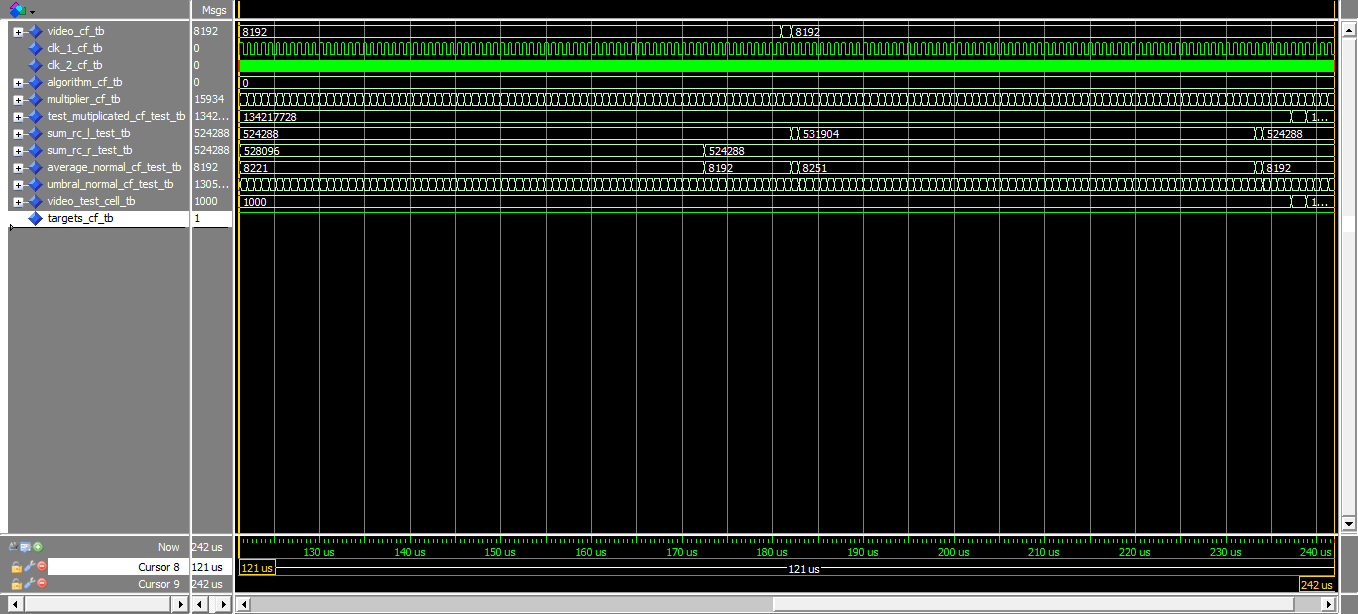
\includegraphics[scale=0.52, angle=270]{./Figures/cfar_ensayo_2.png}
\caption{CFAR. Ensayo 2}
\label{fig:cfar_ensayo_2}
\end{figure}


Se observó resultados similares a los descritos en la sección \ref{Subsec:CFAR. Ensayo 1}. Con diferencias en lo siguiente:

\begin{itemize}
\item
Valores definidas para todas las salidas.

\item
Valor del puerto de salida en nivel alto (1 lógico) durante todo el intervalo de tiempo de ensayo. Esto se debió a que el multiplicador se incrementa linealmente, una unidad en cada flanco ascendente del reloj 1 y hasta el final de la simulación, no adquiere el valor necesario para desplazar el umbral normal por encima del valor máximo del video de entrada.
\end{itemize}



\subsubsection{CFAR. Ensayo 3}
\label{Subsec:CFAR. Ensayo 3}

Se introdujo las señales de estímulo mencionadas en la sección \ref{Subsec:CFAR. Ensayo 1} con diferencia en la señal de video al cfar, compuesta de la siguiente manera:

\begin{itemize}
\item Señal de video de entrada \texttt{video\_cf\_tb} de \texttt{14\-bit} tipo unsigned, periódica de periodo igual a 500 us, con valor \texttt{10000000000000} (8192 en sistema decimal) durante 249.5 us, \texttt{10111011100000} (12000 en sistema decimal) durante 1 us y \texttt{10000000000000} durante 249.5 us.
\end{itemize}

Se simuló el \textit{testbench} del CFAR desde 0 us a 500 us para observar el comportamiento de las sumas de las celdas de referencia, el promedio normal y el umbral normal ante un sólo pulso en un rango de tiempo amplio. El resultado se ilustra en la figura \ref{fig:cfar_ensayo_3}.

\begin{figure}
\centering
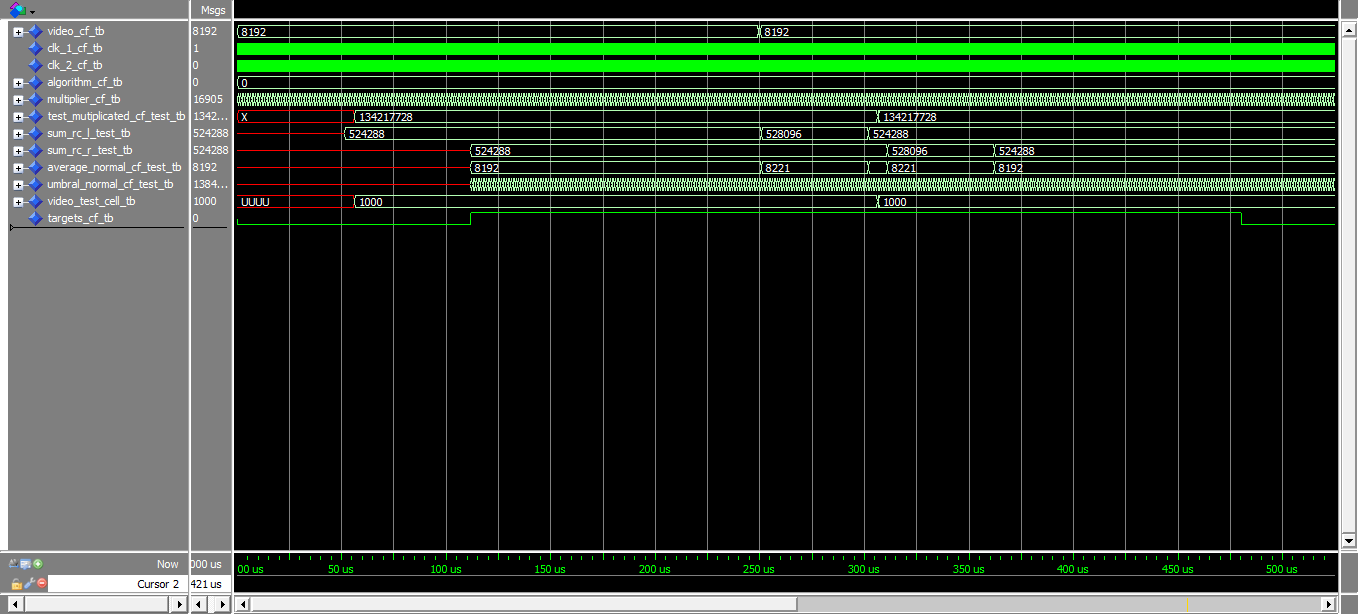
\includegraphics[scale=0.52, angle=270]{./Figures/cfar_ensayo_3.png}
\caption{CFAR.Ensayo 3}
\label{fig:cfar_ensayo_3}
\end{figure}

Se observó una variación escalonada en las señales de salidas correspondiente a ambas sumas de las celdas de referencia y en el promedio normal. Esto fue causado por el recorrido del pulso entre las celdas del CFAR. Se observó que antes y después del paso del pulso, las sumas y el promedio normal se mantienen estables en el valor \texttt{10000000000000} (8192 en sistema decimal). La variación de las sumas se ilustra en la figura \ref{fig:sumas_celdas}. La celda de referencia ubicada a la derecha de la celda test(azul), luego de 60 us, adquiere los mismos valores que la celda de referencia ubicada a la izquierda (rojo).

\begin{figure}
\centering
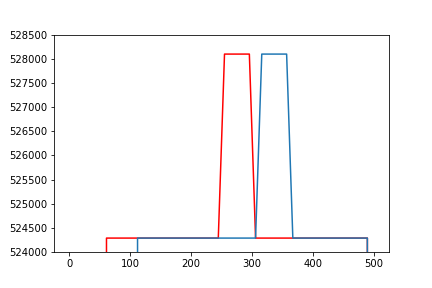
\includegraphics[scale=0.5]{./Figures/cfar_ensayo_3_sumas.png}
\caption{Variación de sumas de celdas de referencia.}
\label{fig:sumas_celdas}
\end{figure}



\subsubsection{CFAR. Ensayo 4}
\label{Subsec:CFAR. Ensayo 4}

Esta simulación comprendió el intervalo de tiempo entre $0 us$ y $7000 us$. El objetivo fue observar la comportamiento de la señal de salida del CFAR correspondiente al target. El resultado se ilustra en la figura \ref{fig:cfar_ensayo_4}.

Se observó que a los $480,47 us$ el multiplicador alcanza el valor $16384$. A partir de ese momento el valor de video almacenado en la celda test superó al umbral sólo en los momentos en donde su valor correspondió al pulso de valor \texttt{10111011100000} (12000 en sistema decimal). Durante toda la simulación el valor del multiplicador se incrementó linealmente, al igual que el umbral normal.

El nivel alto del puerto de salida del CFAR, correspondiente al target, se observó con un comportamiento periódico de acuerdo a lo mencionado en el párrafo anterior. A los $6806.02 us$ la celda test presentó un valor correspondiente al pulso de video, pero no se observó nivel alto del puerto de target debido a que en ese momento el multiplicador alcanzó un valor que incrementó el umbral a un nivel superior al valor máximo del CFAR. Este valor fue $24291$. Teniendo en cuenta la expresión de la ecuación \ref{Eq:Ecuación del umbral normal} y la correción del valor almacenado en la celda bajo testeo, indicada en la ecuación \ref{Eq:corrección_test_cell}, se verificó los datos arrojados en la simulación. Estos valores se ilustran en la figura \ref{fig:cfar_ensayo_4_zoom}, la cual es una imagen ampliada de la figura \ref{fig:cfar_ensayo_4}.

\begin{figure}
\centering
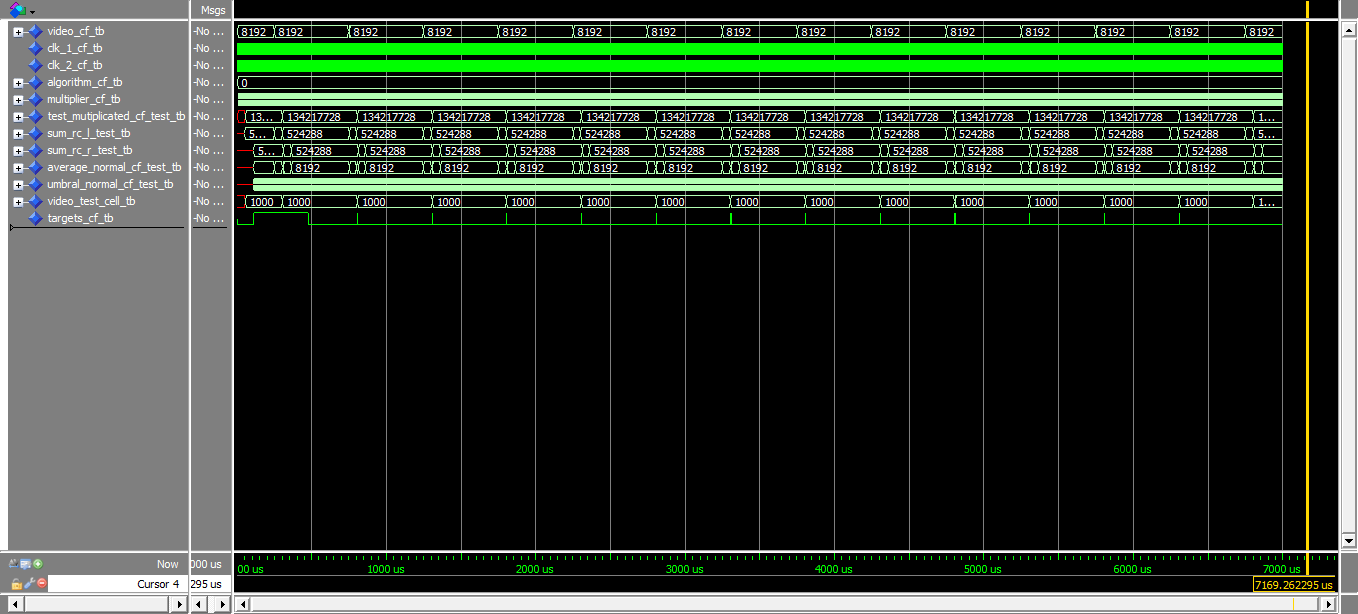
\includegraphics[scale=0.52, angle=270]{./Figures/cfar_ensayo_4.png}
\caption{CFAR.Ensayo 4}
\label{fig:cfar_ensayo_4}
\end{figure}
	
\begin{figure}
\centering
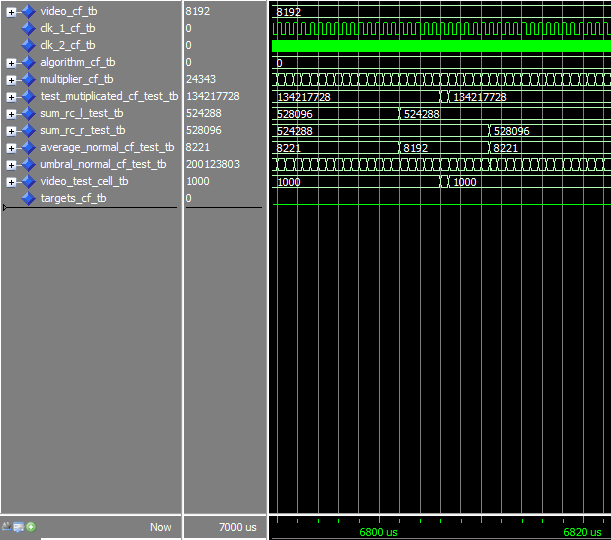
\includegraphics[scale=0.7, angle=0]{./Figures/cfar_ensayo_4_zoom_multiplicador.png}
\caption{CFAR.Ensayo 4. Acercamiento al tiempo $t=6806.02 us$}
\label{fig:cfar_ensayo_4_zoom}
\end{figure}

\subsection{Resultados del Configurador a ensayos con marcos de prueba}


\subsubsection{Configurador. Ensayo 1}
\label{Subsec:Configurador. Ensayo 1}

Se simuló el \textit{test bench} del componente \textit{sectorizador}, instancia del Configurador. El intervalo de simulación estuvo entre $0 us$ y $33 us$. Se introdujo las siguientes señales de estímulo:

\begin{itemize}
\item
\texttt{i\_clk\_tb}: Señal de reloj, de periodo igual a $1 us$.

\item 
\texttt{combinacion\_s}: Señal de $5\-bit$, que incrementó su valor en cada flanco ascendente del reloj y que produjo el efecto de realizar un barrido por todos los sectores.

\item
$32$ señales de multiplicadores, una por cada entrada del sectorizador. Se generó un estímulo que introdujo un valor diferente en cada entrada para evaluar a la salida si el pase por el sector correspondiente se correspondía con la entrada configurada.

\item
$32$ señales de algoritmo, una por cada entrada del sectorizador. Su valor fue \texttt{00} (en sistema binario) para todas las entradas.

\item
$32$ señales de coeficiente de ventana deslizante, una por cada entrada del sectorizador. Su valor fue \texttt{0110} (en sistema binario) para todas las entradas.

\item
$32$ señales de selección de video CFAR, una por cada entrada del sectorizador. Su valor fue $0$ (en sistema binario) para todas las entradas.


\end{itemize}

El tiempo de simulación estuvo comprendido en un intervalo de tiempo entre $0 us$ y $17 us$ para las señales de entrada y salida del multiplicador. Se observó la correcta asignación de los valores a los correspondientes puertos de entrada. Se observó además que salida del multiplicador presentó el valor asignado a cada puerto de entrada luego de dos flancos ascendentes desde el momento en el que el sector actual coincidió numéricamente con el número del puerto de entrada. Por ejemplo, como se ilustra en la figura \ref{fig:cfar_ensayo_1_zoom_multiplicador}, la salida del multiplicador en el tiempo $t = 9 us$, correspondiente al sector actual con valor \texttt{01001} (Sector 10), adquirió el valor \texttt{0000000000001001} de la entrada correspondiente al sector 10, 2 flancos ascendentes después ($10,5 us$) debido al retraso del circuito combinacional. Un análisis similar se puede realizar para las señales restantes debido a que tanto el circuito que proporciona la salida del multiplicador, como los circuitos respectivos de selección de video, algoritmo y coeficiente de ventana deslizante, comparten una arquitectura similar.

\begin{figure}
\centering
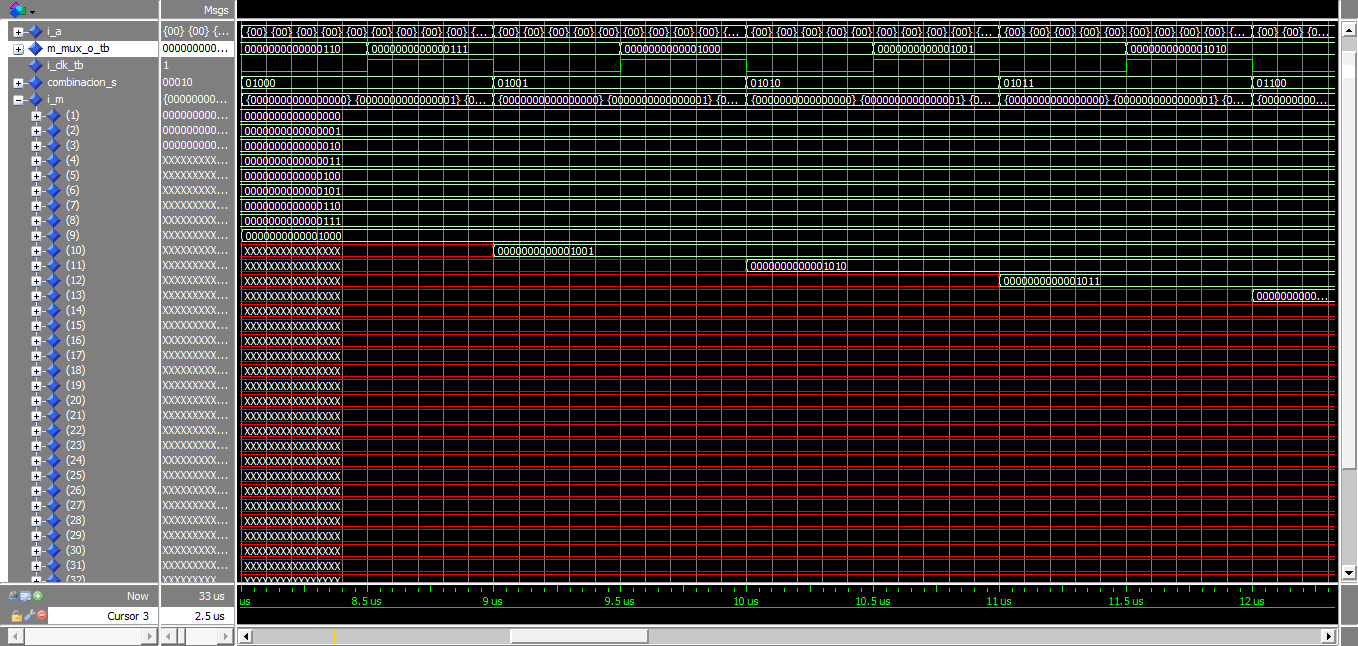
\includegraphics[scale=0.5, angle=270]{./Figures/sectorizador_ensayo_1_zoom_mult.png}
\caption{Sectorizador. Ensayo 1. Acercamiento alrededor de $t = 9us$.}
\label{fig:sectorizador_ensayo_1_zoom_mult}
\end{figure}


\begin{itemize}
\item
Valor bajo equivalente al piso de ruido durante todo el periodo, excepto durante un pequeño intervalo de tiempo en la que adquiere un valor mayor. Se eligió como valor bajo \texttt{10000000000000} debido a que el conversor de alta velocidad es de 14-bit signado y el valor mencionado corresponde al cero. Físicamente el piso de ruido era cercano a cero. El valor de amplitud del pulso de video se eligió \texttt{10111011100000} como valor cercano al $50\%$ del rango de operación.


\item
Periódica de periodo suficientemente largo para que exista un solo pulso en el intervalo de tiempo que comprende la totalidad de celdas CFAR. La totalidad de las celdas CFAR generan un retardo indicado en la ecuación \ref{Eq:delay_cfar}, donde $N_{rc}$ es igual al número total de las celdas de referencia (128), $N_{gc}$ es igual al número total de las celdas de guarda (10) y $N_t$ es igual a el número total de las celdas bajo testeo (1).

\end{itemize}






\subsubsection{Configurador. Ensayo 2}
\label{Subsec:Configurador. Ensayo 2}
Se simuló el \textit{test bench} del componente \textit{ajuste de multiplicador}, instancia del Configurador. El intervalo de simulación estuvo entre $0 us$ y $22 us$. Se introdujo las siguientes señales de estímulo:

\begin{itemize}

\item
\texttt{i\_decision\_tb}: Señal de decisión, con valor inicial \texttt{01}, \texttt{10} luego de $3 us$, \texttt{00} luego de $13 us$ y \texttt{01} luego de $19 us$.

\item
\texttt{i\_sub\_mode\_tb}: Configuración de submodo, con valor inicial \texttt{0} y \texttt{1} luego de $2.5 us$.

\item
\texttt{i\_clk\_tb}: Señal de reloj, de periodo igual a $1 us$.

\item
\texttt{i\_rst\_tb}: Señal de reset, con valor constante $0$.

\item
\texttt{i\_multiplier\_tb}: Señal de multiplicador, con valor constante \texttt{11110000000000} ($15360$ en sistema decimal).

\end{itemize}

\begin{figure}
\centering
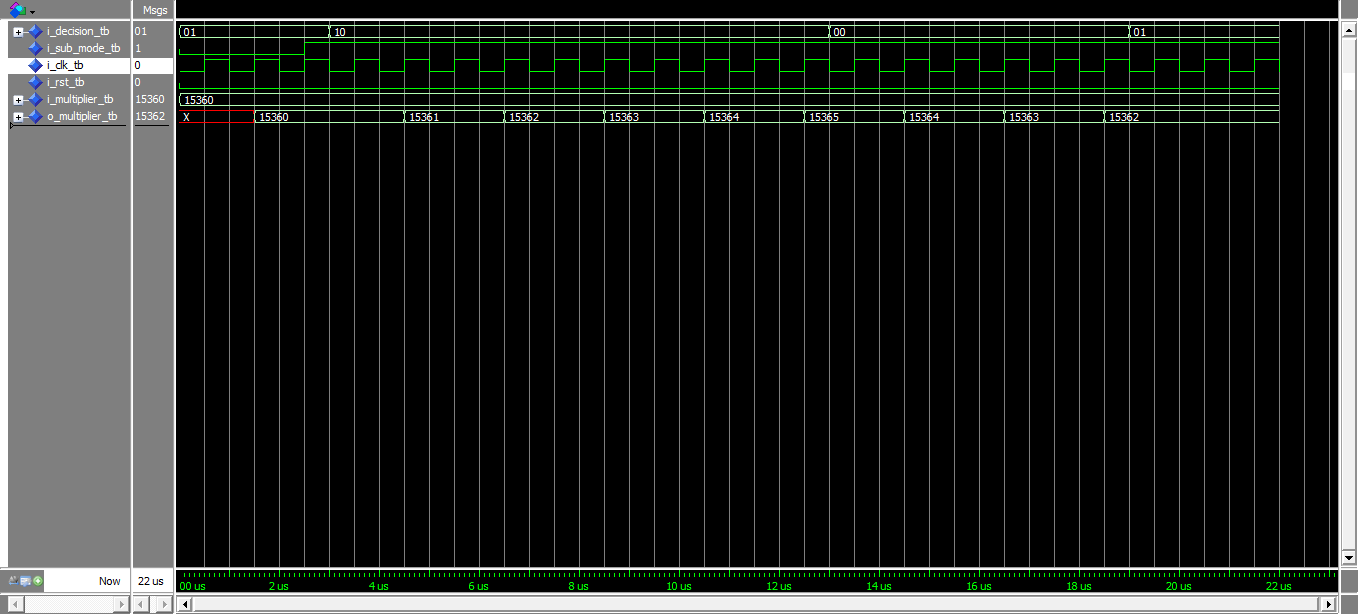
\includegraphics[scale=0.52, angle=270]{./Figures/multiplier_setting_ensayo_1.png}
\caption{Configurador. Ensayo 2}
\label{fig:multiplier_setting_ensayo_1}
\end{figure}

El resultado se ilustra en la figura \ref{fig:multiplier_setting_ensayo_1}. Un valor de decisión \texttt{01} significa "no realizar modificaciones al multiplicador", en otras palabras: dejar ese valor constante. Un valor de decisión \texttt{10} significa \"incrementar el valor del multiplicador en un delta". Donde el \textit{delta} tuvo valor $1$ por defecto. Por último, un valor de decisión \texttt{00} significa "decrementar el valor del multiplicador en un delta". La señal del multiplicador de entrada es constante debido a que el mismo se almacena en un registro externo al módulo e interno a cada sector, se toma dicho valor como referencia.

Se observó que para $t = 1.5 us$, luego de $2$ flancos ascendentes de reloj, la salida queda definida en el valor configurado desde la entrada. Este valor se mantiene constante entre $t = 1.5 us$ y $t = 3 us$, intervalo de tiempo en el que el submodo estuvo con valor $0$ correspondiente a una operación fija. A partir de $t = 3 us$ el submodo adquirió valor $1$ indicando una operación automática, esto significa que se habilita con una modificación automática del último valor del multiplicador almacenado en el registro interno al módulo en función del valor de decisión de entrada. Se observó que entre $t = 3 us$ y $t = 13 us$, intervalo de tiempo en donde la decisión tomó valor $10$, el valor del multiplicador aumentó en una unidad en cada flanco ascendente de reloj. Para el intervalo de tiempo entre $t = 13 us$ y $t = 19 us$, donde la decisión tomó valor $00$, el valor del multiplicador disminuyó en una unidad en cada flanco ascendente de reloj. Finalmente, a partir de $t = 19 us$, con el valor de decisión $01$, el valor del multiplicador permaneció constante.



\subsubsection{Configurador. Ensayo 3}
\label{Subsec:Configurador. Ensayo 3}
Se simuló el \textit{test bench} del Configurador. El intervalo de simulación estuvo entre $0 us$ y $40 us$. Se introdujo las siguientes señales de estímulo:

\begin{itemize}
\item
Para el bloque fijo:
	\begin{itemize}
	\item
	\texttt{i\_multiplier\_fxs\_tb}: Señal de multiplicador, con valor constante de \texttt{1110000000000000}.
	
	\item
	\texttt{i\_algorithm\_fxs\_tb}: Señal de algoritmo, con valor constante de \texttt{00}.   
	
	\item  
	\texttt{i\_window\_sliding\_fxs\_tb}: Señal de coeficiente de ventana deslizante, con valor constante de \texttt{0000}.
	
	\item
	\texttt{i\_tolerancia\_fxs\_tb}: Señal de tolerancia, con valor constante de \texttt{00101}.    

	\end{itemize}

\item
Para un sector en particular:
	\begin{itemize}
  	\item
  	\texttt{i\_algortihm\_cfar\_tb}: Señal de algoritmo con valor \texttt{00} durante los primeros $11 us$, luego \texttt{10}.
  
  	\item
  	\texttt{i\_sub\_mode\_tb}: Señal de submodo con valor constante \texttt{0} (modo fijo).
  
  	%\item
  	%\texttt{i_presence_required_tb}. Comento porque no interesa para éste ensayo.
  
  	\item
  	\texttt{i\_multiplier\_cfar\_tb}: Señal de multiplicador, con valor \texttt{1110000000000000} durante los primeros $11 us$, luego \texttt{1111000000000001}.
  
  	\item
  	\texttt{i\_window\_sliding\_tb}: Señal de coeficiente de ventana deslizante, con valor \textit{0100} durante los primeros $11 us$, luego \texttt{1010}.
  
  	\item
  	\texttt{i\_sector\_addr\_tb}: Señal de identificación de sector, con valor \texttt{00101} durante los primeros $11 us$, luego \texttt{00011}.
	\end{itemize}

\item
Señales comunes:
	\begin{itemize}
	\item
	\texttt{i\_clk\_tb}: Señal de reloj, de periodo igual a $1 us$.
	
	\item 
	\texttt{combinacion\_s}: Señal de $5\-bit$, que incrementó su valor en cada flanco ascendente del reloj y que produjo el efecto de realizar un barrido por todos los sectores.
	
    
    \item
    \texttt{i\_mode\_tb}: Señal de modo de operación, con valor \texttt{0} (no sectorizado) durante los primeros $10 us$, luego \texttt{1} (sectorizado).
    
    \item
    \texttt{i\_load\_config\_tb}: Señal de carga de configuración a un sector determinado, consiste en un pulso de una duración de $1 us$. Se generó dos pulsos de carga de configuración, el primero a los $2 us$ y el segundo a los $13 us$.
    
    \item
    \texttt{i\_tolerancia\_tb}: Señal de modo de tolerancia, con valor constante \texttt{10} (2 en sistema decimal).
    
    \item
    \texttt{i\_passed\_through\_north\_tb}: Señal de paso por el norte, consiste en un pulso de una duración de $1 us$. Se utilizó esta señal para actualizar la salida de todos los sectores del modo sectorizado. Se generó dos pulsos de paso por el norte, el primero a los $7 us$ y el segundo a los $18 us$. Es necesario que estos pulsos se produzcan después de  el pulso de carga de configuración para que la salida presente el valor configurado con el pulso de carga mencionado.
	\end{itemize}

\end{itemize}



\begin{figure}
\centering
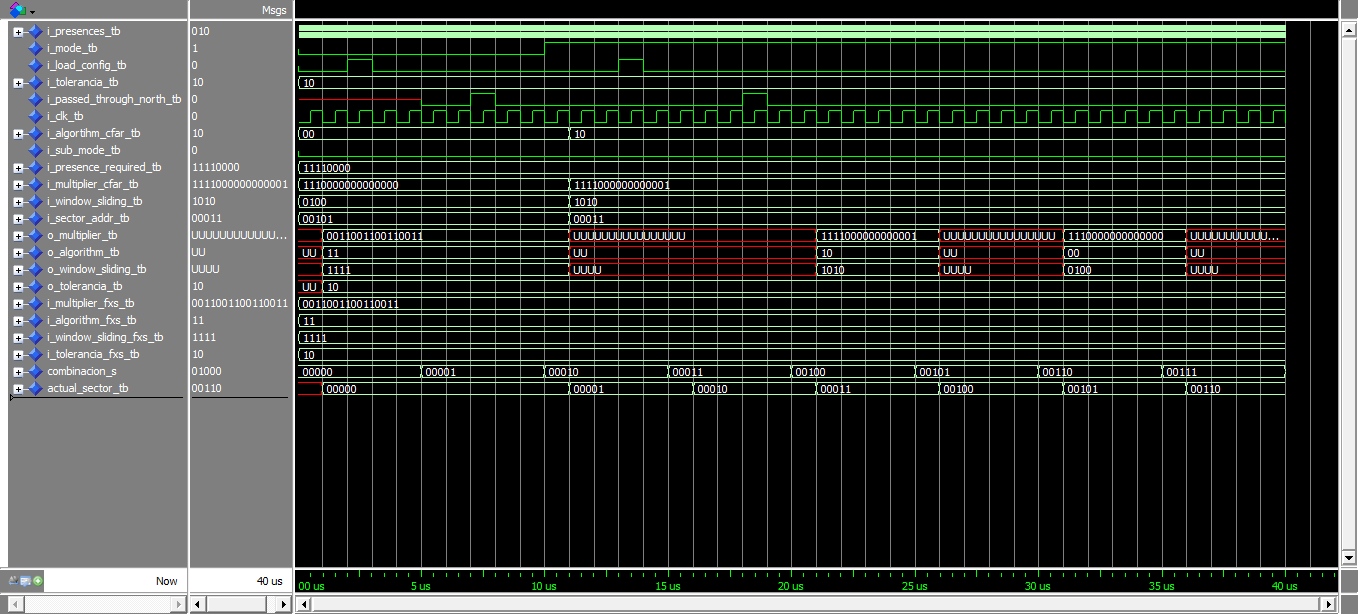
\includegraphics[scale=0.52, angle=270]{./Figures/configurador_ensayo_3.png}
\caption{Configurador. Ensayo 3}
\label{fig:configurador_ensayo_3}
\end{figure}


El resultado se ilustra en la figura \ref{fig:configurador_ensayo_3}. Se observó que durante los primeros $10 us$ la señal de modo permanece en $0$. Debido a esto la salida de los sectores con \textit{id} \texttt{00000} y \texttt{00001} son ignoradas mientras el sector actual adquiere estos valores, en cambio la salida del configurador adopta los valores de multiplicador, algoritmo, coeficiente de ventana y tolerancia del sector fijo. Esta salida tiene lugar desde el tiempo $t = 1 us$ en el flanco descendente del reloj, estando indefinida por este motivo en el momento inicial. Cabe mencionar que para asegurar la estabilidad de los datos al momento de la lectura por parte del CFAR, se eligió para la salida del configurador como flanco activo el flanco descendente. De esta manera se produce un desfase entre la actualización del dato a la salida de este módulo y la lectura del dato a la entrada del CFAR.

Luego de los $10 us$ se observó que la señal de modo conmutó a $1$. Esto produce un cambio en la salida del configurador. En modo sectorizado se ignora la salida del sector fijo y se considera la salida de los $32$ sectores restantes, proporcionando a la salida del configurador la configuración almacenada para el sector correspondiente al sector actual. Debido a que se configuró sólo dos sectores, se observó que la salida del configurador estuvo indefinida para aquellos sectores que no fueran los que se configuraron.

En $t = 21 us$, cuando el sector actual cambia de valor de \texttt{00010} y \texttt{00011}, las salidas del configurador adpotan los valores configurados para el sector \texttt{00011} de acuerdo a los estímulos generados. Una situación similar ocurre para $t = 21 us$ con el sector \texttt{00101}



\subsubsection{Resultados a ensayos con visores de netlist}
\label{Subsec: Resultados de Visores de netlist}

\begin{figure}
\centering
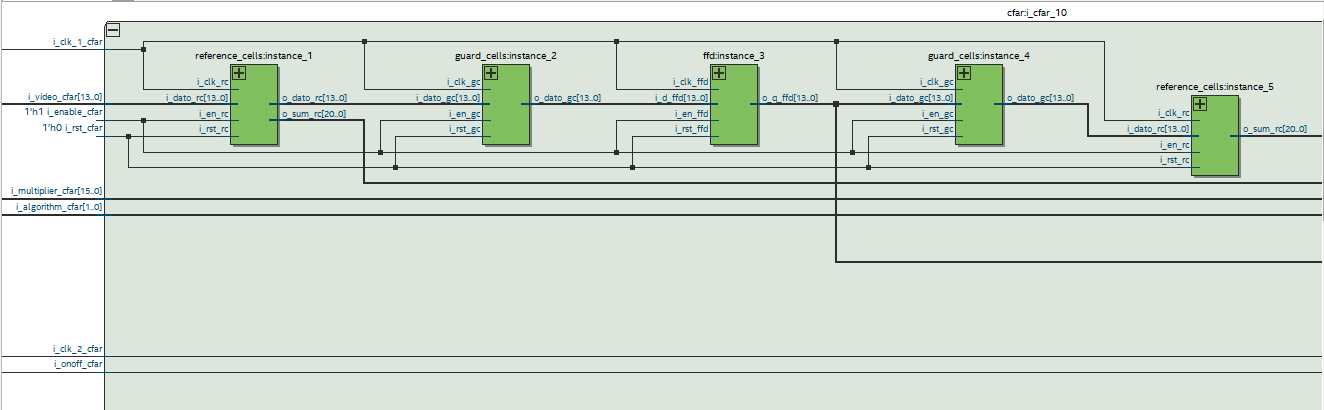
\includegraphics[scale=0.6, angle=270]{./Figures/RTL_cfar_1.png}
\caption{Diagrama RTL de la sección de entrada del módulo CFAR}
\label{fig:RTL_cfar_1}
\end{figure}


\begin{figure}
\centering
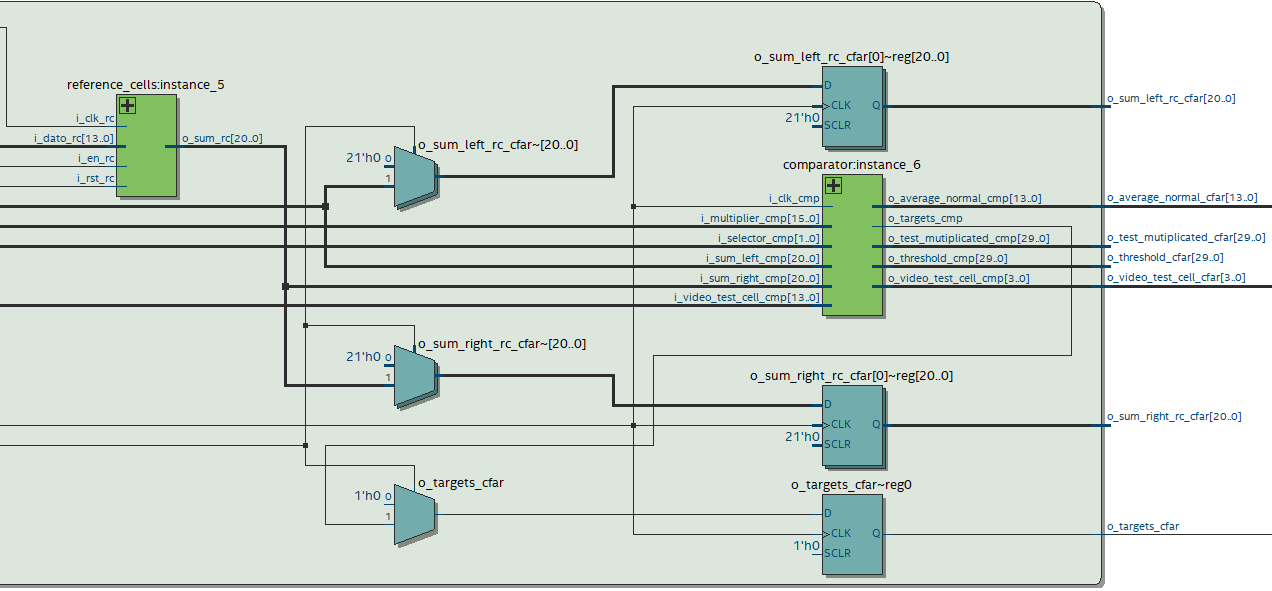
\includegraphics[scale=0.5]{./Figures/RTL_cfar_2.png}
\caption{Diagrama RTL de la sección de salida del módulo CFAR}
\label{fig:RTL_cfar_2}
\end{figure}



\begin{figure}
\centering
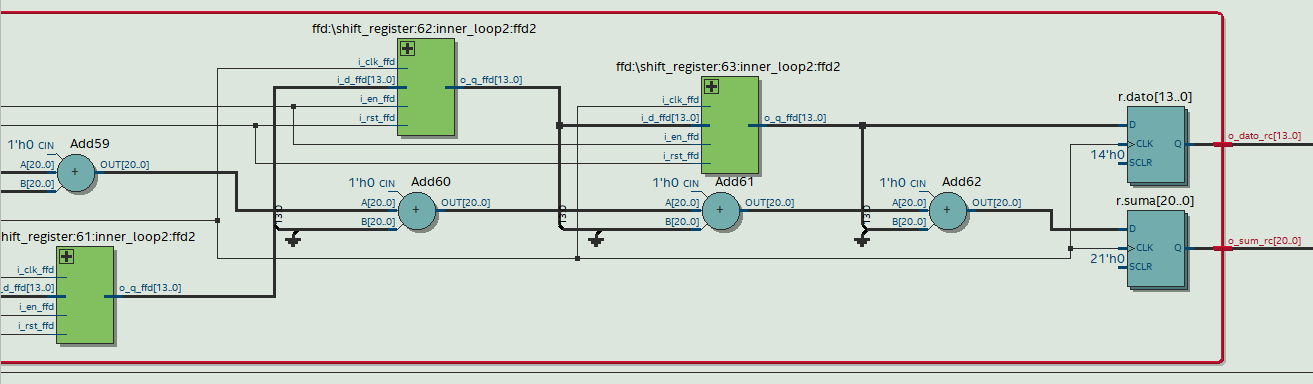
\includegraphics[scale=0.6, angle=270]{./Figures/RTL_cfar_rc_1.png}
\caption{Diagrama RTL de la sección de salida de una celda de referencia}
\label{fig:RTL_cfar_rc_1}
\end{figure}



\begin{figure}
\centering
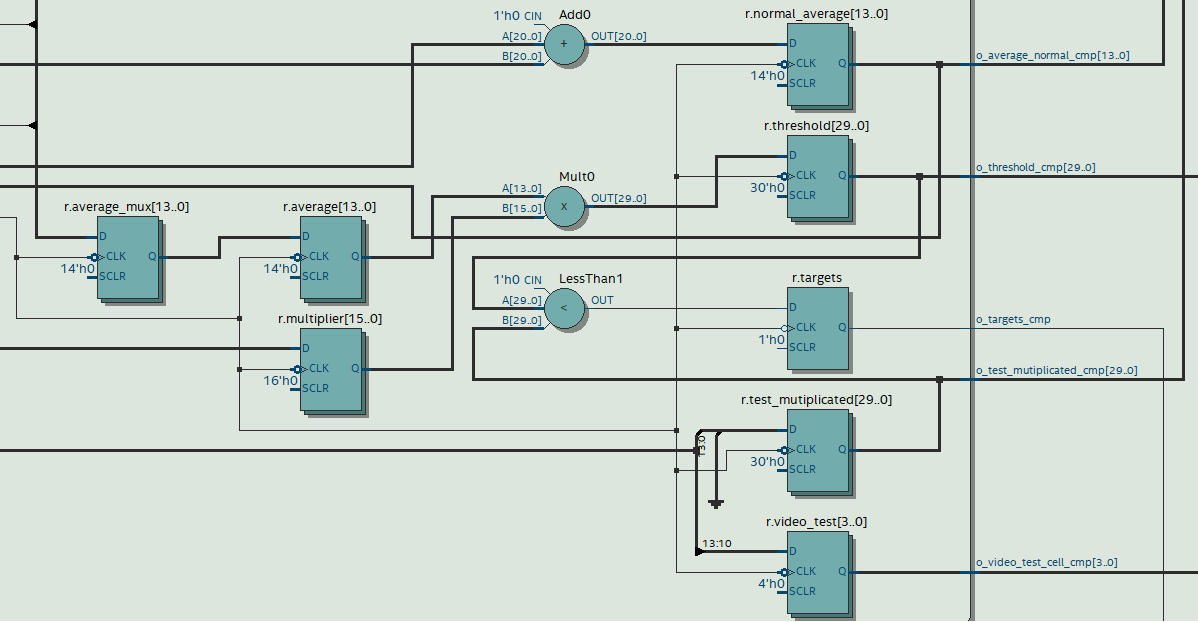
\includegraphics[scale=0.6, angle=270]{./Figures/RTL_cfar_comparador_1.png}
\caption{Diagrama RTL de la sección de salida del comparador}
\label{fig:RTL_cfar_comparador_1}
\end{figure}






\begin{figure}
\centering
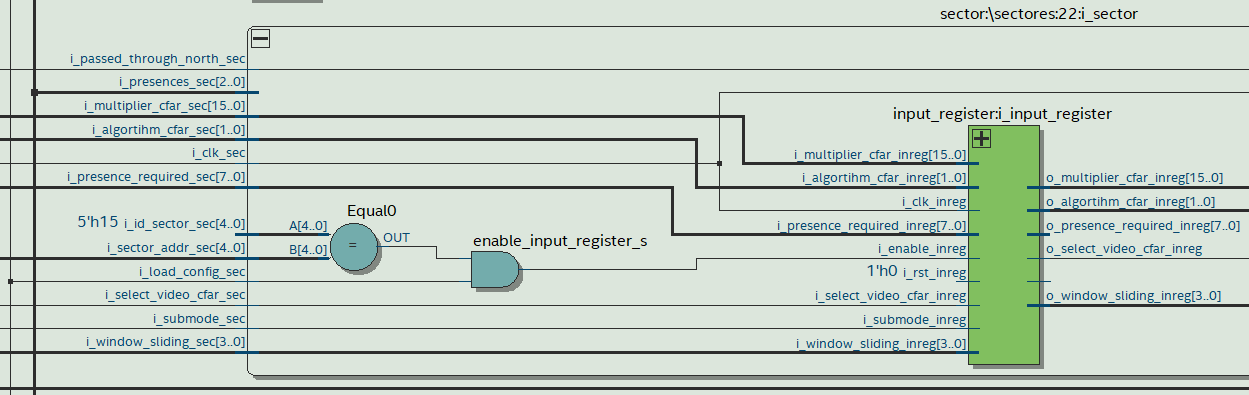
\includegraphics[scale=0.65, angle=270 ]{./Figures/RTL_cfg_sector_1.png}
\caption{Diagrama RTL de la sección de entrada de un sector}
\label{fig:RTL_cfg_sector_1}
\end{figure}



\begin{figure}
\centering
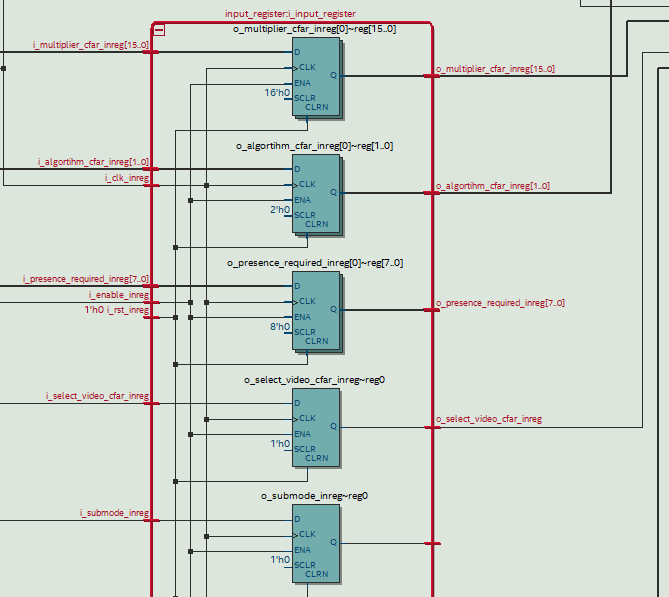
\includegraphics[scale=0.75]{./Figures/RTL_cfg_input_reg_1.png}
\caption{Diagrama RTL de una sección del registro de entrada interno a un sector}
\label{fig:RTL_cfg_input_reg_1}
\end{figure}




Se compiló el diseño del Procesador Monoradar, el cual incluyó como subsistemas a los módulos CFAR y Configurador. Superada la etapa de análisis y síntesis, fue posible utilizar la herramienta \textit{RTL Viewer} para verificar la interpretación de la herramienta de síntesis, del código RTL compilado.

Se observó el esquema RTL de las celdas CFAR, el cual se ilustra en la figura \ref{fig:RTL_cfar_1}. Los registros de desplazamientos se conectaron adecuadamente. Se verificó que todos fueron conectados a la misma fuente de reloj y compartieron las señales de habilitación y reset. Estas características permiten, según el fabricante, una adecuada inferencia de los registros de desplazamiento como tales y por tanto permiten que se efectúen procesos de optimización sobre el diseño. Se verificó además que exista una conexión serie entre estos registros. En cuanto a la sección de salida del CFAR, se verificó las conexiones del comparador y la interpretación, por parte de la herramienta de síntesis, de la lógica combinacional y secuencial de salida. Se ilustra en la figura \ref{fig:RTL_cfar_2}, los registros y \textit{flip flop} inferidos por la herramienta de síntesis a la salida del módulo CFAR. La herramienta de síntesis interpretó una lógica intermedia entre las señales provenientes de las celdas CFAR o el comparador y los registros de salida, para las señales de targets y de suma. Esta lógica consistió en una compuerta \texttt{AND} esquematizada con un multiplexor.

Desplegando uno de los módulos correspondientes a las celdas de referencia, se observó la estructura interna de esos módulos. La sección de salida se ilustra en la figura \ref{fig:RTL_cfar_rc_1}. Se observó una conexión serie de los registros, una conexión de sumadores en cascada y dos registros de salida para almacenar la suma y el video. En particular la conexión de sumadores en cascada permitió la escalabilidad del módulo; fue posible durante el diseño generar celdas de referencia con diferente cantidad de celdas sin mayores complicaciones.

Para el componente \textit{comparador} se observó la interpretación por parte de la herramienta de síntesis de un circuito combinacional y otro secuencial, acorde a la descripción realizada en la sección \ref{metodologia_estructurada} del capítulo \ref{Chapter2} sobre la \textit{metodología estructurada}. En la figura \ref{fig:RTL_cfar_comparador_1} se ilustra la sección de salida del comparador compuesta por un circuito secuencial.

En cuanto al configurador, se verificó la interpretación de la descripción RTL del módulo. Se ilustran ejemplos de los esquemas RTL del sector y del registro de entrada interno al sector, en las figuras \ref{fig:RTL_cfg_sector_1} y \ref{fig:RTL_cfg_input_reg_1}. En la figura \ref{fig:RTL_cfg_sector_1} se ilustra la condición de igualdad que debe cumplirse entre la señal de combinación de sector y la señal de identificación de ese sector, luego con una compuerta \textit{AND} se impuso otra condición para que se habilite la carga de la configuración con una señal adicional (proveniente del puente HPS). En la figura \ref{fig:RTL_cfg_input_reg_1} se ilustra parte de los diferentes componentes que componen el módulo: por un lado \textit{flip flops} tipo D para la selección del video CFAR y el submodo, y por el otro registros para la presencia requerida, algoritmo y multiplicador.
